\documentclass{report}
\usepackage{pdfpages}
\usepackage[a4paper, top=2cm, bottom=2cm, left=2cm, right=2cm]{geometry}
\usepackage{fancyhdr}
\usepackage{amsmath} % Für mathematische Symbole
\usepackage{amssymb} % Für \mathbb
\usepackage[linesnumbered,ruled]{algorithm2e} % Für Algorithmus-Umgebung
\usepackage{ulem}
\usepackage{xcolor}
\usepackage{array}
\usepackage{graphicx}
\usepackage{listings}
\usepackage{xcolor}
\usepackage{naive-ebnf}
\usepackage[utf8]{inputenc}
\usepackage[absolute,overlay]{textpos}
\usepackage{tcolorbox}

\lstdefinestyle{cppstyle}{
    language=C++,             % Specify the language
    basicstyle=\ttfamily,     % Set the font to typewriter
    basicstyle=\ttfamily\footnotesize,
    keywordstyle=\color{blue}\bfseries, % Keywords in bold blue
    commentstyle=\color{green},         % Comments in green
    stringstyle=\color{red},            % Strings in red
    numbers=left,            % Line numbers on the left
    numberstyle=\tiny\color{gray}, % Line numbers in tiny gray font
    stepnumber=1,             % Line number step
    breaklines=true,          % Automatic line breaking
    tabsize=4,                % Set tab size
    showstringspaces=false,   % Don't show spaces in strings
    frame=single,             % Add a frame around the code
}

\newcommand{\name}{Marco Söllinger}
\newcommand{\fach}{SEN2}
\newcommand{\topic}{Übung 1}
\newcommand{\uebungangabe}{Uebung1.pdf}

\newcommand{\matnr}{s2410306011}
\newcommand{\uebungsgruppe}{Gruppe 1}
\newcommand{\aufwand}{4}


\pagestyle{fancy}
\normalem 
\fancyhead[R]{Marco Söllinger}  

\begin{document}
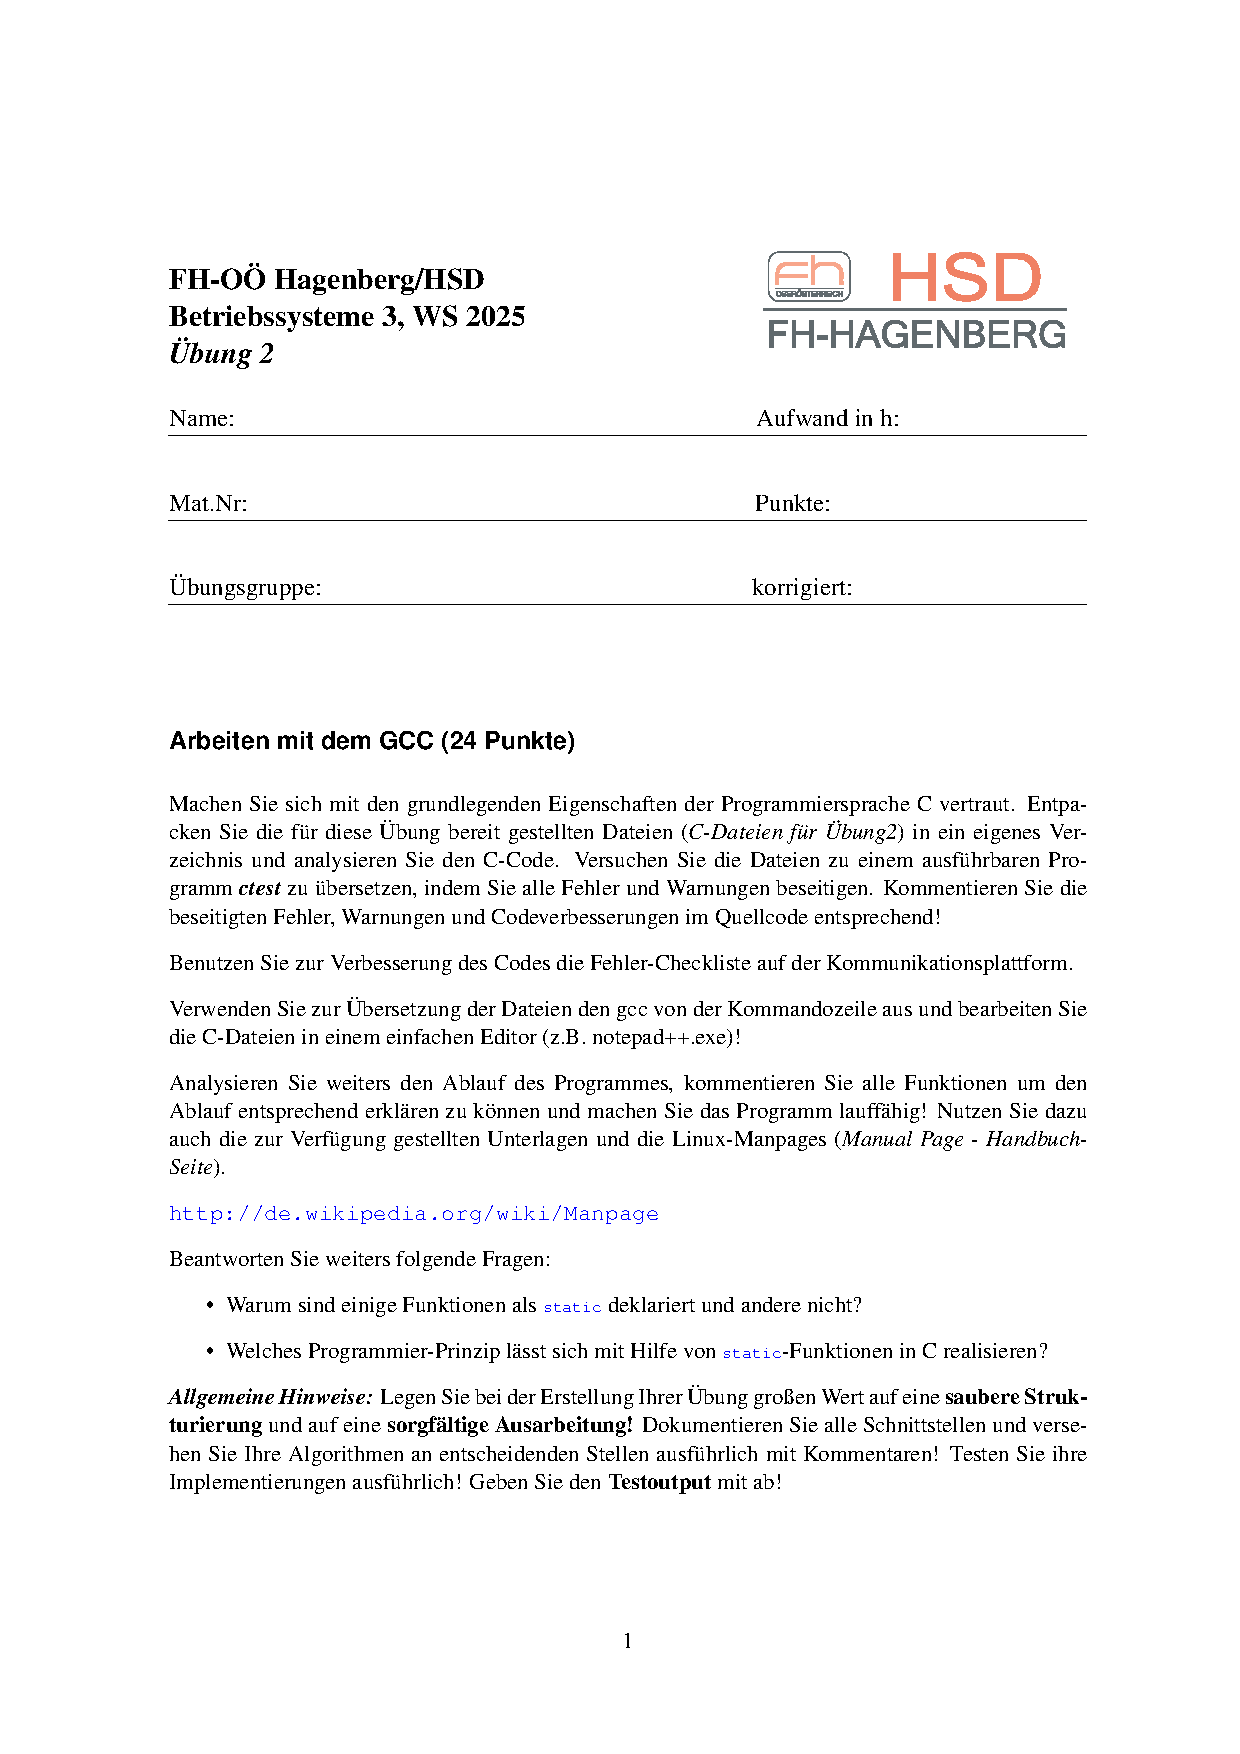
\includepdf[pages=1,pagecommand={
			\begin{textblock*}{5cm}(5.5cm, 6.9cm)
				\textbf{\name}
			\end{textblock*}
			\begin{textblock*}{5cm}(5.5cm, 8.4cm)
				\textbf{\matnr}
			\end{textblock*}
			\begin{textblock*}{5cm}(5.5cm, 9.8cm)
				\textbf{\uebungsgruppe}
			\end{textblock*}
			\begin{textblock*}{5cm}(15.3cm, 6.9cm)
				\textbf{\aufwand}
			\end{textblock*}
		}]{Uebung2.pdf}
%\includepdf[pages=2-]{Uebung2.pdf}

\section*{Beispiel 1}
Es wurde wie in der Aufgabenstellung verlangt das C Programm korregiert, sodass es ohne Warnungen kompiliert.\\
Fuer das compilieren wurde folgendes Kommando verwendet:\\
gcc main.c Print.c Test.c -o cTest -Wall -Wextra -Werror\\\\
Die Aenderungen wurden in dem Code kommentiert.\\\\

\subsection*{1.1 Code}

\lstinputlisting[style=cppstyle, title=\texttt{main.c} ]{../c_testprog2/main.c}
\lstinputlisting[style=cppstyle, title=\texttt{Print.h} ]{../c_testprog2/Print.h}
\lstinputlisting[style=cppstyle, title=\texttt{Print.c} ]{../c_testprog2/Print.c}
\lstinputlisting[style=cppstyle, title=\texttt{Test.h} ]{../c_testprog2/Test.h}
\lstinputlisting[style=cppstyle, title=\texttt{Test.c} ]{../c_testprog2/Test.c}

\subsection*{1.2 Test}

\begin{lstlisting}[style=cppstyle, title=\texttt{Terminal Output}]
flashfish@fedora ~/D/R/F/B/U/c_testprog2 (main)> ./cTest

Test Format IO
==============
i: 1 Address: 0x7fff22a531ec
Bitte eingeben: 1
1

Geben sie einen Integer ein:2
2
0x7fff22a531e8
A
PI: 3.141500
Format IO Test OK


Test Strings
============
Length of "Das ist ein C-String" is 20 chars
Buffer: Das ist ein C-String
Text vorher : ABC
Text nachher: CAB
String Test OK


Test dynamic Memory
===================
 -> Hello World!
Memory Test OK


Test Structs
============
Person: Max Mustermann hat 80 kg
Person: Moritz Mustermann hat 80 kg
Struct Test OK


initialized array with 0:
=========================
0
0
0
0
0
0
0
0
0
0

initialized array with 1:
=========================
16843009
16843009
16843009
16843009
16843009
16843009
16843009
16843009
16843009
16843009
Array Test OK


Test Function Pointers
======================
Anton
Berta
Hello
Martha
notnA
atreB
olleH
ahtraM
Length of "Anton" is 5 chars
Length of "Berta" is 5 chars
Length of "Hello" is 5 chars
Length of "Martha" is 6 chars
FuncPtr Test OK
\end{lstlisting}

\section*{Beispiel 2}

\subsection*{1 Frage: Warum sind einige Funktionen als static deklariert?}
Das keyword static bei Funktionen sorgt dafuer, dass der Linker weiss, dass diese Funktion nur in der jeweiligen .c sichbar sein soll.\\
Es sichert also, internal linkage zu. Wenn man dies nicht macht, koennte man mit dem keyword extern in anderen .c Dateien auf diese Funktion zugreifen.\\
Static verhindert also Namenskonflikte und sorgt fuer eine bessere Kapselung.\\\\
Generell kann man sagen, dass alle Funktionen, die nicht in der .h Datei deklariert sind, static sein sollten.\\

\subsection*{2 Frage: Welches Programmier-Prinzip laesst sich mit Hilfe von static-Funktionen umsetzen?}
Mit static Funktionen laesst sich also Information Hiding umsetzen, bzw man kann damit private Funktionen von der Objektorientierung nachstellen\\

\end{document}
